\documentclass[beamer]{BetterDocument}

\beamerBackground{img/background.jpg}

\definecolor{titlecolor}{HTML}{FFFFFF}
\definecolor{titlebg}{HTML}{4db6ac}
\definecolor{sectionBg}{HTML}{26a69a}

\title{Magic Book}
\author{DEROUIN Auréline 21806986\\
	MARTIN Justine 21909920}
\institute{UniCaen}
\date{2019 - 2020}

\begin{document}

	\frame{\titlepage}

	\begin{frame}
		\frametitle{Table des matières}
		\tableofcontents
	\end{frame}

	\section{Présentation de l'application}
	\begin{frame}
		\frametitle{L'interface d'édition}
		\begin{graphicsRow}
			\graphicsCol{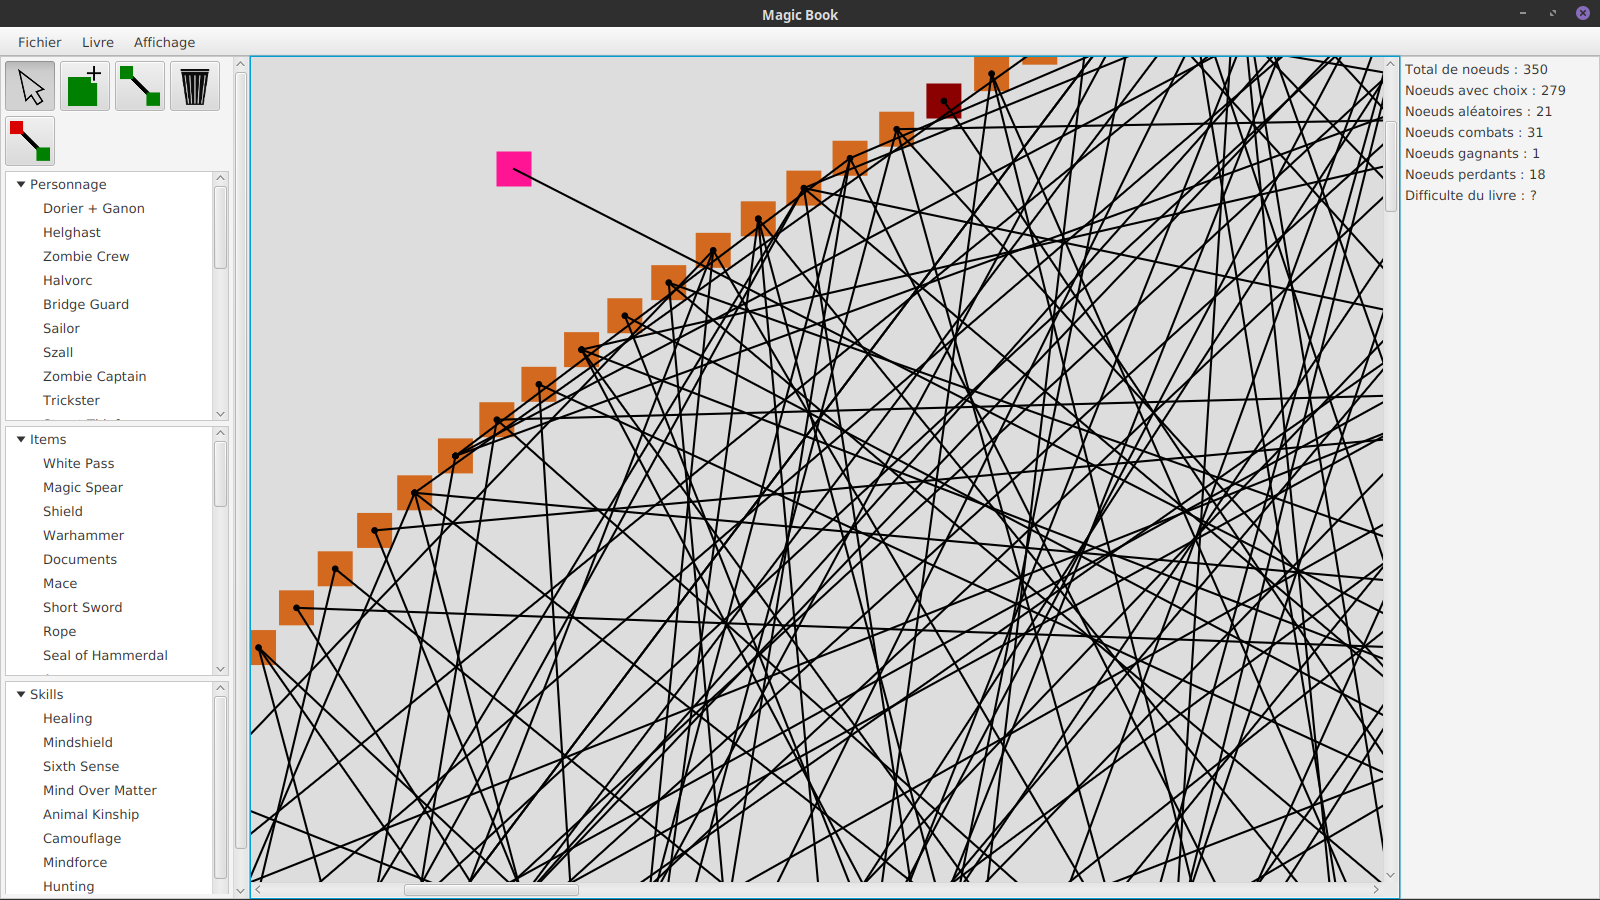
\includegraphics[width=0.5\paperwidth, keepaspectratio]{img/editeur.png}}
			\hfill
	        \graphicsCol{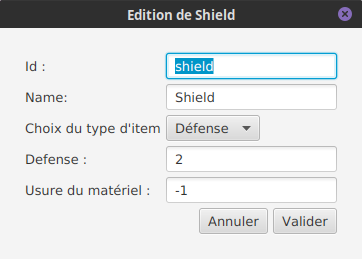
\includegraphics[width=0.3\paperwidth, keepaspectratio]{img/editeur_item.png}}
		\end{graphicsRow}
	\end{frame}

	\begin{frame}
		\frametitle{Le mode jeu}
		\begin{graphicsRow}
			\graphicsCol{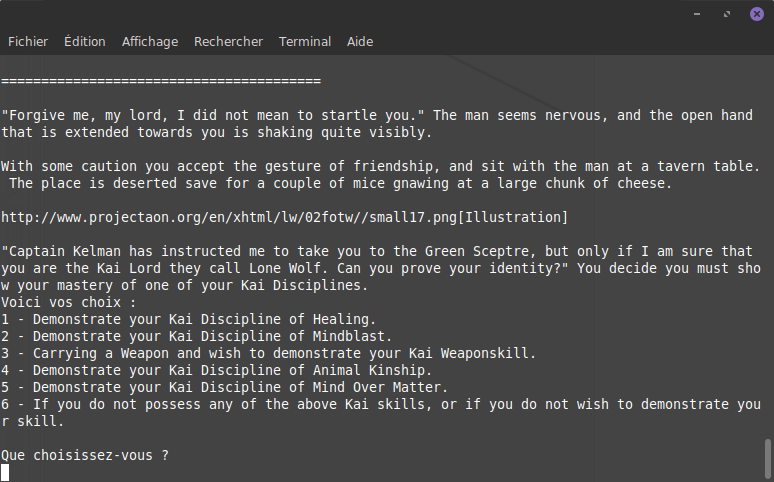
\includegraphics[width=0.45\paperwidth, keepaspectratio]{img/jeu_choix.png}}
			\hfill
	        \graphicsCol{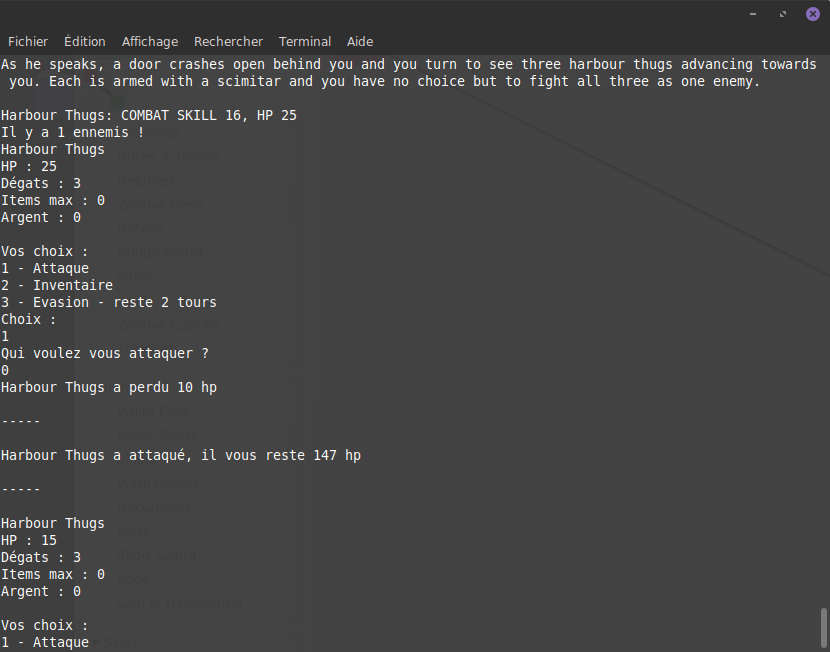
\includegraphics[width=0.38\paperwidth, keepaspectratio]{img/jeu_combat.png}}
		\end{graphicsRow}
	\end{frame}

	\section{Estimation de la difficulté d'un livre}
	\subsection{Fonctionnement}
	\begin{frame}
		\frametitle{L'idée d'origine}
	\end{frame}

	\begin{frame}
		\frametitle{Les améliorations apportées}
	\end{frame}

	\subsection{Problèmes et idées d'amélioration}
	\begin{frame}
		\frametitle{Les points noirs actuels}
	\end{frame}

	\begin{frame}
		\frametitle{Pistes de réflexions}
	\end{frame}

\end{document}
